%
% psigraph.tex -- Psi Funktion für erstes Wavelet-Transformation Beispiel
%
% (c) 2019 Prof Dr Andreas Müller, Hochschule Rapperswil
%
\documentclass[tikz]{standalone}
\usepackage{amsmath}
\usepackage{times}
\usepackage{txfonts}
\usepackage{pgfplots}
\usepackage{csvsimple}
\usetikzlibrary{arrows,intersections,math}
\begin{document}
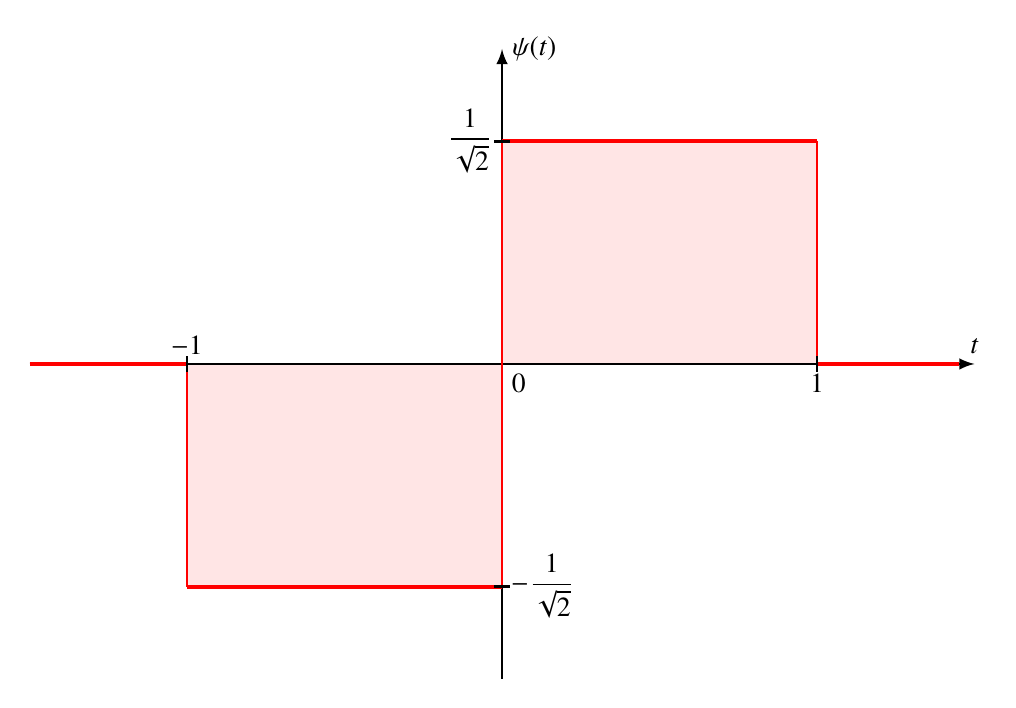
\begin{tikzpicture}[>=latex,scale=4]

\fill[color=red!10] (0,0) rectangle (1,{1/sqrt(2)});
\fill[color=red!10] (0,0) rectangle (-1,{-1/sqrt(2)});

\draw[->,line width=0.9pt] (-1.5,0)--(1.5,0) coordinate[label={$t$}];
\draw[->,line width=0.9pt] (0,-1)--(0,1) coordinate[label={right:$\psi(t)$}];

\draw[color=red,line width=1.4pt] (-1,{-1/sqrt(2)})--(0,{-1/sqrt(2)});
\draw[color=red,line width=1.4pt] (0,{1/sqrt(2)})--(1,{1/sqrt(2)});
\draw[color=red,line width=1pt] (-1,0)--(-1,{-1/sqrt(2)});
\draw[color=red,line width=1pt] (0,{-1/sqrt(2)})--(0,{1/sqrt(2)});
\draw[color=red,line width=1pt] (1,{1/sqrt(2)})--(1,0);
\draw[color=red,line width=1.4pt] (-1.5,0)--(-1,0);
\draw[color=red,line width=1.4pt] (1,0)--(1.45,0);

\draw[line width=1pt] (1,-0.025)--(1,0.025);
\draw[line width=1pt] (-1,-0.025)--(-1,0.025);
\draw[line width=1pt] (-0.025,{1/sqrt(2)})--(0.025,{1/sqrt(2)});
\draw[line width=1pt] (-0.025,{-1/sqrt(2)})--(0.025,{-1/sqrt(2)});

\node at (1,0) [below] {$1$};
\node at (-1,0) [above] {$-1$};
\node at (0,{1/sqrt(2)}) [left] {$\displaystyle\frac1{\sqrt{2}}$};
\node at (0,{-1/sqrt(2)}) [right] {$\displaystyle-\frac1{\sqrt{2}}$};
\node at (0,0) [below right] {$0$};

\end{tikzpicture}
\end{document}

